\begin{tikzpicture}[actor/.append style={minimum width=2.5cm, text width=2.3cm}]
  \Actores{cli/1.45/{Equipo\\ del Cliente},des/4.65/{Despacho\\ (solicitante y firmante)},api/8.0/{API},tsa/11.3/{TSA local},pg/14.6/{PostgreSQL}}{-15.0}
  \Msg{4.65}{8.0}{-1.1}{\textbf{1} versión, partes, vigencia y folio}
  \Paso{8.0}{-1.25}{2.7}{Valida partes y vínculos y fija \texttt{CTRTREQ1}}
  \Msg{8.0}{14.6}{-2.55}{solicitud y aviso}
  \Msg[msgR]{8.0}{1.45}{-3.25}{\textbf{2} solicitud, PDF, certificados y declaración 1}
  \Paso{1.45}{-3.4}{2.7}{Recalcula las huellas, compara campo a campo y firma con su clave}
  \Msg{1.45}{8.0}{-5.2}{\textbf{3} firma S1, sin la clave}
  \Msg{8.0}{11.3}{-5.85}{T1 sobre la huella de S1}
  \Msg[msgR]{11.3}{8.0}{-6.4}{sello}
  \Paso{8.0}{-6.55}{2.7}{Comprueba la vigencia con el instante de T1}
  \Paso[pasoError]{11.3}{-6.55}{2.4}{Falla: no deja estado; reenvío explícito}
  \Msg{8.0}{14.6}{-7.85}{\textbf{4} firma, evento y avisos}
  \Msg[msgR]{8.0}{1.45}{-8.5}{acuse parcial}
  \Msg[msgR]{8.0}{4.65}{-9.15}{\textbf{5} declaración 2 con las huellas de S1 y T1}
  \Paso{4.65}{-9.3}{2.7}{Valida el acuse parcial y firma con su clave}
  \Msg{4.65}{8.0}{-10.75}{\textbf{6} firma S2}
  \Msg{8.0}{11.3}{-11.4}{Td sobre el PDF y Tf sobre el manifiesto}
  \Msg[msgR]{11.3}{8.0}{-11.95}{sellos}
  \Paso{8.0}{-12.1}{2.7}{Exige T1 $\le$ Td $\le$ Tf y la vigencia}
  \Paso[pasoError]{4.65}{-12.1}{2.7}{Certificado del Cliente revocado en la CRL: se rechaza}
  \Msg{8.0}{14.6}{-13.55}{\textbf{7} firma, compleción y evento}
  \Paso{14.6}{-13.7}{2.3}{Una sola transacción}
  \Msg[msgR]{8.0}{1.45}{-14.55}{paquete completo para ambas partes}
\end{tikzpicture}
